\documentclass[tikz]{standalone}
\usepackage{tikz}
\usetikzlibrary{positioning, graphs}
\usetikzlibrary{graphs.standard}
\begin{document}
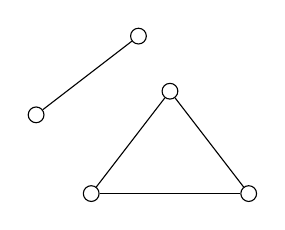
\begin{tikzpicture}
		[every node/.style={draw,circle,inner sep = 0mm, minimum size = 2mm}]
		\node at (0.3,0) (a) {};
		\node at (1.6,1) (b) {};
		\node at (1,-1) (c) {};
		\node at (3,-1) (e) {};
		\node at (2,0.3) (f) {};
		
        \draw (a) -- (b);
        \draw (c) -- (f);
        \draw (e) -- (c);
        \draw (f) -- (e);
\end{tikzpicture}
\end{document}